\documentclass{article}
\usepackage[utf8]{inputenc}
\usepackage[spanish]{babel}
\usepackage[colorlinks]{hyperref}
\usepackage{graphicx}

\begin{document}
\begin{titlepage}
    \centering
    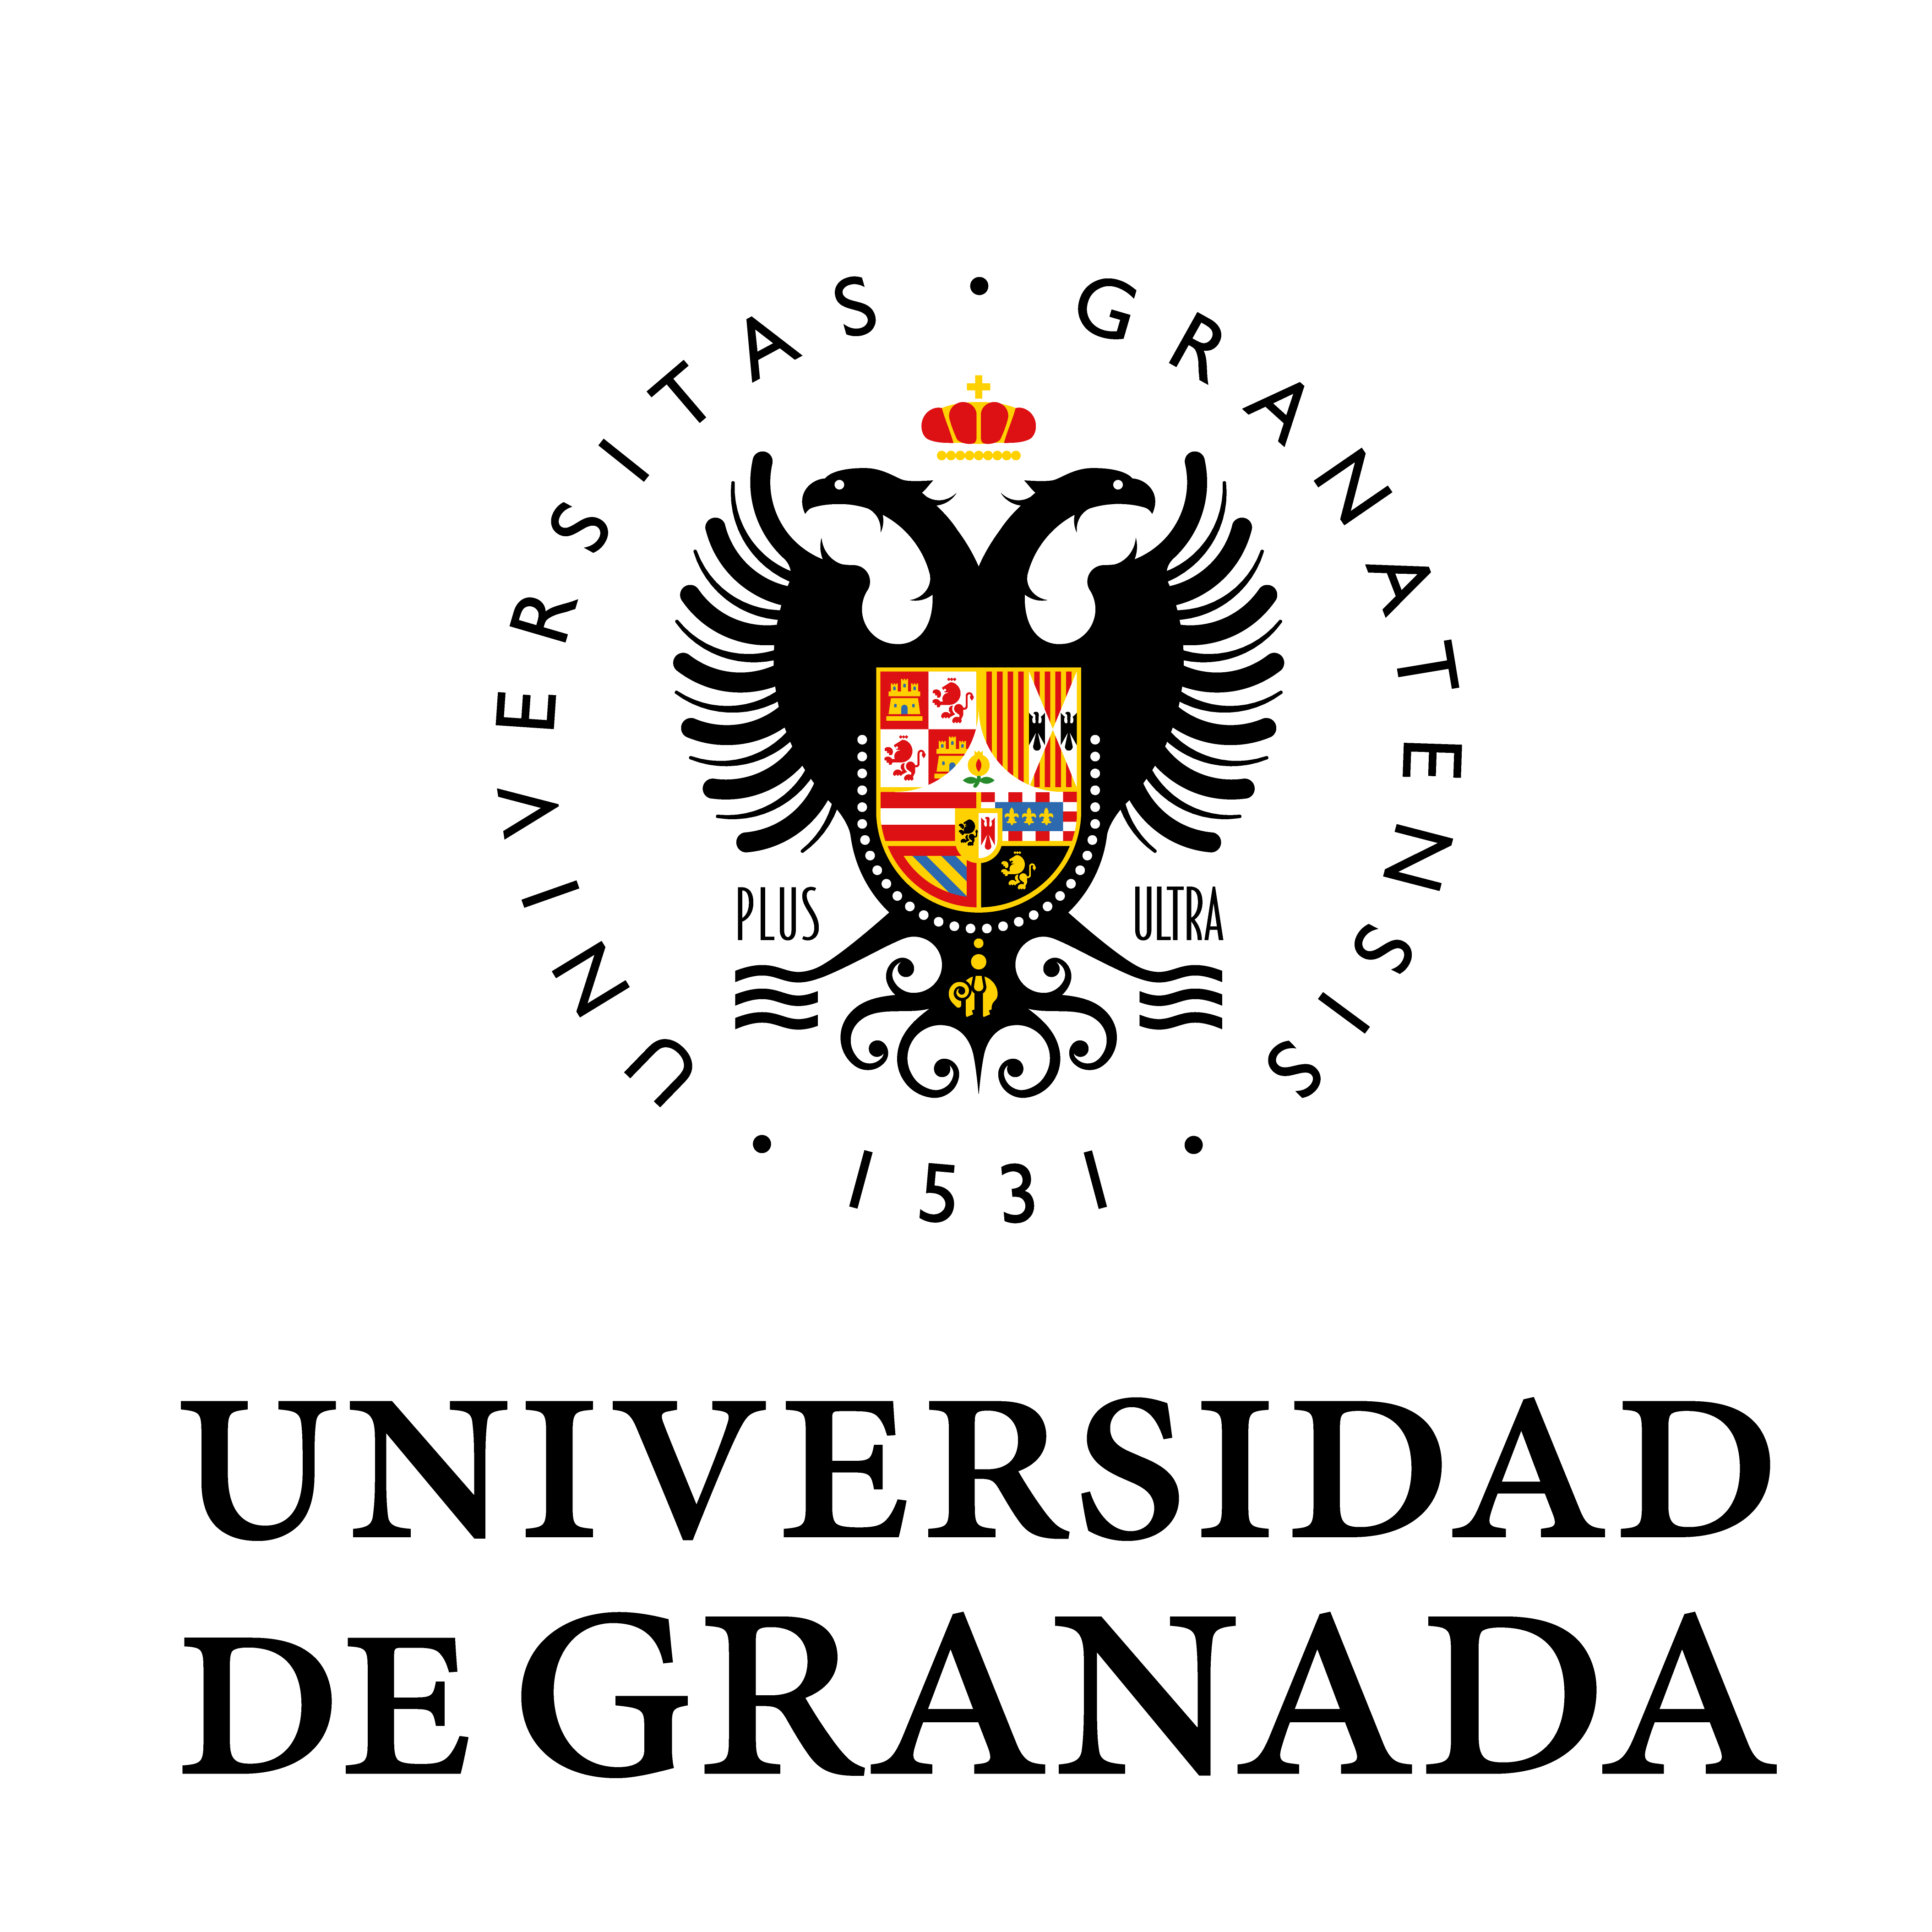
\includegraphics[width=0.5\textwidth]{images/logo-ugr.png}\par
    \vspace{1cm}
    {\Large\scshape Entornos Virtuales \par}
    {\huge\bfseries Simulación \par}
    \vspace{0.2cm}
    {\scshape Práctica 5 \par}
    \vfill
    {\large Víctor Vázquez Rodríguez  \par}
    {victorvazrod@correo.ugr.es \par}
    \vfill
    {\large Máster Universitario en Ingeniería Informática \par}
    \vspace{0.2cm}
    {Curso 2019/20 \par}
\end{titlepage}

Esta práctica se centra en la adición de físicas a la escena que se ha venido
preparando en las prácticas anteriores. Para poder reflejar los distintos
aspectos de las físicas que se han expuesto para esta práctica, he comenzado
creando un vagón de carga que se une a la locomotora para formar un tren. Este
vagón y su unión con la locomotora se pueden ver en la Figura \ref{fig:wagon}.

Se han definido las físicas de ambas jerarquías de objetos de forma que las
partes externas (cuerpo, ruedas, frenos) calculan colisiones, mientras que las
internas (panel de control de la locomotora) no. Las piezas que se usan para el
enganche entre la locomotora y el vagón tampoco tienen colisiones ya que no es
necesario. En cuanto al tipo de físicas, la locomotora es \textit{dynamic},
mientras que el vagón es \textit{rigid body}.

Para que no haya problemas entre los objetos de una misma jerarquía, se han
usado grupos de colisiones (uno para la locomotora y otro para el vagón) y la
opción \textit{compound} de la configuración, de forma que solo se calculan
colisiones con otros objetos y no entre ellos.

La principal razón por la que se ha incorporado el vagón es para incluir una
restricción de tipo bisagra o \textit{hinge} en la escena: la locomotora y el
vagón se unen usando una de estas restricciones, permitiendo al vagón pivotar en
un eje. El centro de este pivote se ha desplazado para que se ubique en la unión
de los enganches de las dos partes y se ha movido el eje x (el de pivote de la
bisagra) para que el movimiento sea el correcto. Esto se puede ver en la Figura
\ref{fig:pivot}.

Para que el tren no caiga al vacío al lanzar el motor de juegos, se ha colocado
un plano estático debajo y se le ha aplicado una textura de césped para que haga
de escenario. Por último, se han añadido una serie de rocas y una pelota. Las
rocas son de tipo \textit{rigid body} y caen dentro del vagón al lanzar el motor
de juegos, constituyendo así la carga del tren. La pelota, por otra parte, es de
tipo \textit{soft body} para que se deforme como lo haría una pelota real. En la
Figura \ref{fig:final} se puede apreciar la escena final que se ha creado.

\begin{figure}
    \centering
    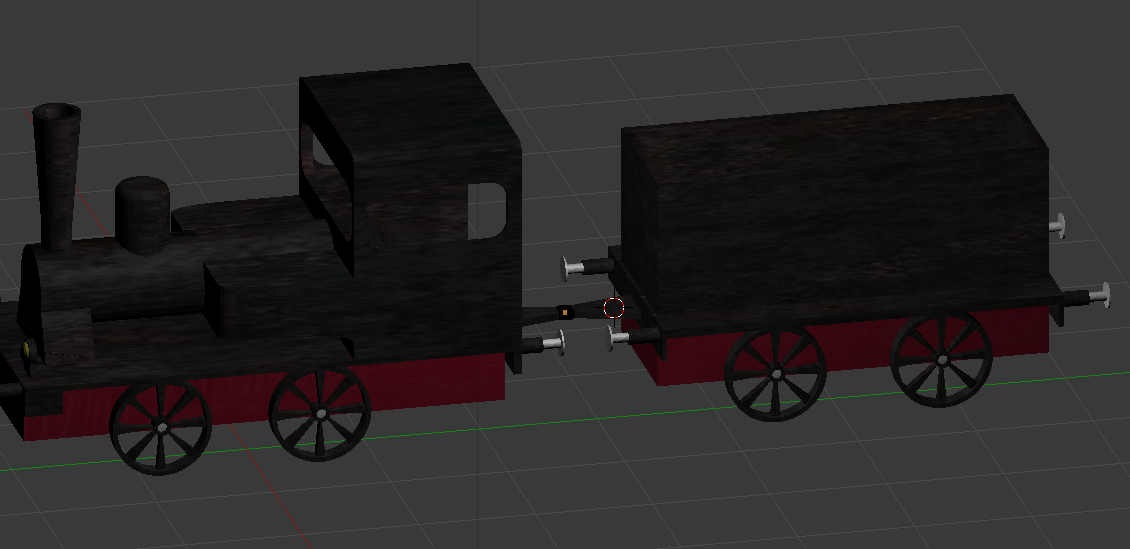
\includegraphics[width=\textwidth]{images/wagon.png}
    \caption{Vagón de carga añadido al tren}
    \label{fig:wagon}
\end{figure}

\begin{figure}
    \centering
    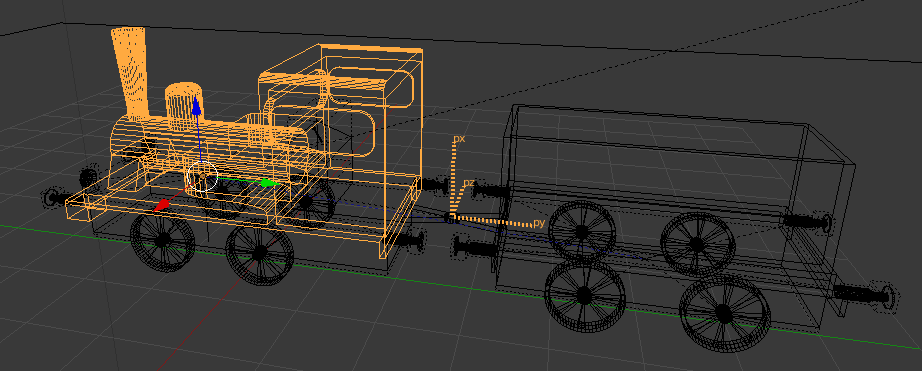
\includegraphics[width=\textwidth]{images/pivot.png}
    \caption{Ejes de rotación de la bisagra}
    \label{fig:pivot}
\end{figure}

\begin{figure}
    \centering
    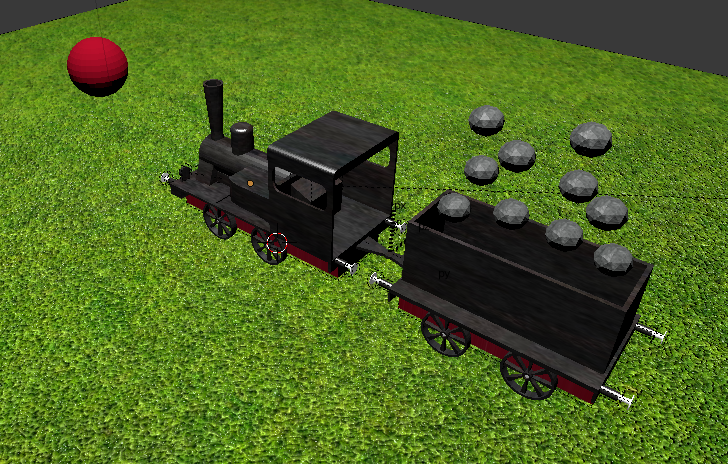
\includegraphics[width=\textwidth]{images/final.png}
    \caption{Escena final con las rocas y la pelota}
    \label{fig:final}
\end{figure}

\end{document}
